

\begin{center}
\thispagestyle{empty}
%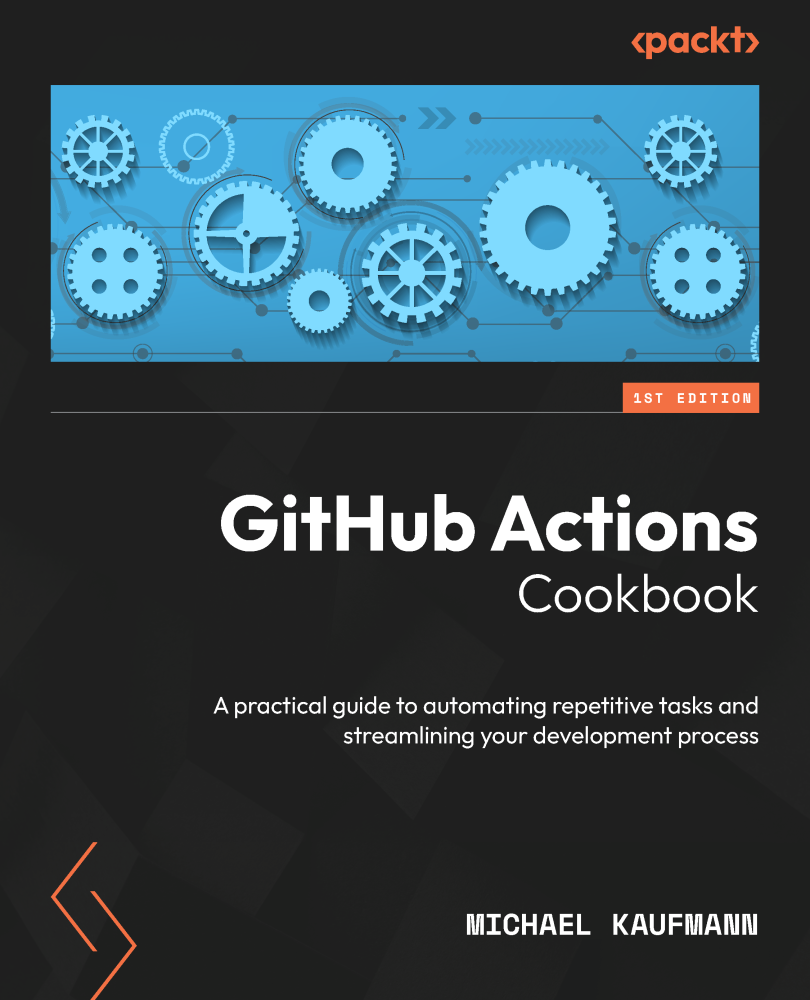
\includegraphics[width=\textwidth,height=\textheight,keepaspectratio]{cover.png}
\begin{tikzpicture}[remember picture, overlay, inner sep=0pt]
\node at (current page.center)
{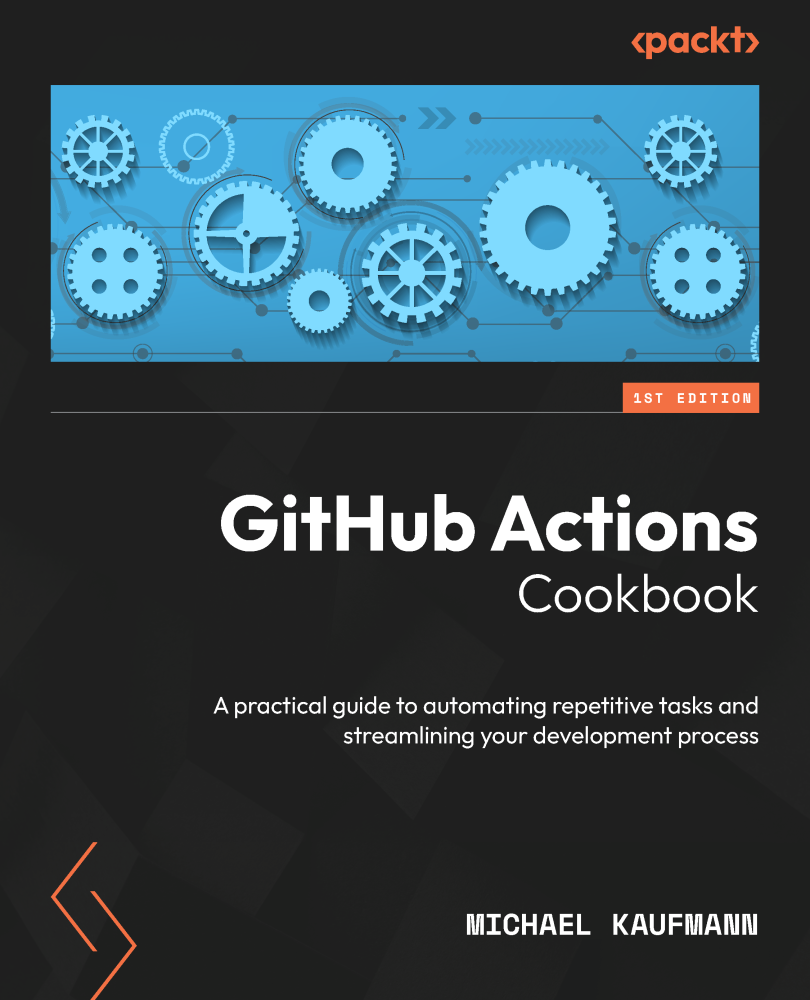
\includegraphics[width=\paperwidth, keepaspectratio=false]{cover.png}};
\end{tikzpicture}
\newpage
\thispagestyle{empty}
\huge
\textbf{GitHub Actions 实用指南}
\\[9pt]
\normalsize
自动化重复任务和优化开发流程
\\[9pt]
\normalsize
作者: Michael Kaufmann
\\[8pt]
\normalsize
译者:\href{https://github.com/xiaoweiChen/GitHub-Actions-Cookbook}{陈晓伟}
\\[8pt]
\end{center}

\newpage

\begin{comment}
\end{comment}

\pagestyle{empty}
\tableofcontents
\newpage

\setsecnumdepth{section}

\myChapter{关于作者}{}{content/about-the-author.tex}
\newpage

\myChapter{前言}{}{content/preface.tex}
\newpage

\myChapter{第1章}{GitHub动作工作流}{content/chapter1/0.tex}
\mySubsection{1.1.}{环境要求}{content/chapter1/1.tex}
\mySubsection{1.2.}{GitHub生态系统}{content/chapter1/2.tex}
\mySubsection{1.3.}{Github的托管和定价}{content/chapter1/3.tex}
\mySubsection{1.4.}{GitHub Actions的价格}{content/chapter1/4.tex}
\mySubsection{1.5.}{GitHub 市场}{content/chapter1/5.tex}
\mySubsection{1.6.}{使用工作流编辑器编写工作流}{content/chapter1/6.tex}
\mySubsection{1.7.}{使用密钥和变量}{content/chapter1/7.tex}
\mySubsection{1.8.}{创建和使用环境}{content/chapter1/8.tex}
\newpage

\myChapter{第2章}{编写和调试工作流}{content/chapter2/0.tex}
\mySubsection{2.1.}{环境要求}{content/chapter2/1.tex}
\mySubsection{2.2.}{使用Visual Studio Code编写工作流}{content/chapter2/2.tex}
\mySubsection{2.3.}{分支中开发工作流}{content/chapter2/3.tex}
\mySubsection{2.4.}{检查工作流}{content/chapter2/4.tex}
\mySubsection{2.5.}{将消息写入日志}{content/chapter2/5.tex}
\mySubsection{2.6.}{启用调试记录}{content/chapter2/6.tex}
\mySubsection{2.7.}{本地运行工作流}{content/chapter2/7.tex}
\newpage

\myChapter{第3章}{构建 GitHub Actions}{content/chapter3/0.tex}
\mySubsection{3.1.}{环境要求}{content/chapter3/1.tex}
\mySubsection{3.2.}{创建Docker容器操作}{content/chapter3/2.tex}
\mySubsection{3.3.}{添加输出参数并使用作业摘要}{content/chapter3/3.tex}
\mySubsection{3.4.}{创建 TypeScript 操作}{content/chapter3/4.tex}
\mySubsection{3.5.}{创建复合操作}{content/chapter3/5.tex}
\mySubsection{3.6.}{在复合操作中使用 github-script 为issue添加评论}{content/chapter3/6.tex}
\mySubsection{3.7.}{将操作共享到市场}{content/chapter3/7.tex}
\newpage

\myChapter{第4章}{工作流的运行时}{content/chapter4/0.tex}
\mySubsection{4.1.}{环境要求}{content/chapter4/1.tex}
\mySubsection{4.2.}{设置自托管运行器}{content/chapter4/2.tex}
\mySubsection{4.3.}{自动扩展自托管运行器}{content/chapter4/3.tex}
\mySubsection{4.4.}{使用 ARC 通过 Kubernetes 实现自托管运行器的扩展}{content/chapter4/4.tex}
\mySubsection{4.5.}{运行器与运行器组}{content/chapter4/5.tex}
\mySubsection{4.6.}{GitHub 托管的运行器}{content/chapter4/6.tex}
\newpage

\myChapter{第5章}{使用 GitHub Actions 在 GitHub 中自动化任务}{content/chapter5/0.tex}
\mySubsection{5.1.}{环境要求}{content/chapter5/1.tex}
\mySubsection{5.2.}{创建issue模板}{content/chapter5/2.tex}
\mySubsection{5.3.}{使用 GitHub CLI 和 GITHUB\_TOKEN 访问资源}{content/chapter5/3.tex}
\mySubsection{5.4.}{使用环境进行审批和检查}{content/chapter5/4.tex}
\mySubsection{5.5.}{可重用工作流和复合操作}{content/chapter5/5.tex}
\newpage

\myChapter{第6章}{构建并验证代码}{content/chapter6/0.tex}
\mySubsection{6.1.}{环境要求}{content/chapter6/1.tex}
\mySubsection{6.2.}{构建和测试代码}{content/chapter6/2.tex}
\mySubsection{6.3.}{使用矩阵构建不同版本}{content/chapter6/3.tex}
\mySubsection{6.4.}{通知用户有关构建和测试结果的详细信息}{content/chapter6/4.tex}
\mySubsection{6.5.}{使用CodeQL查找安全漏洞}{content/chapter6/5.tex}
\mySubsection{6.6.}{创建发布并发布软件包}{content/chapter6/6.tex}
\mySubsection{6.7.}{软件包的版本控制}{content/chapter6/7.tex}
\mySubsection{6.8.}{生成和使用 SBOM(软件物料清单)}{content/chapter6/8.tex}
\mySubsection{6.9.}{工作流中使用缓存}{content/chapter6/9.tex}
\newpage

\myChapter{第7章}{使用 GitHub Actions 发布软件}{content/chapter7/0.tex}
\mySubsection{7.1.}{环境要求}{content/chapter7/1.tex}
\mySubsection{7.2.}{构建并发布容器}{content/chapter7/2.tex}
\mySubsection{7.3.}{使用 OIDC 安全地部署到任何云}{content/chapter7/3.tex}
\mySubsection{7.4.}{环境审批检查}{content/chapter7/4.tex}
\mySubsection{7.5.}{将容器应用程序发布到 AKS}{content/chapter7/5.tex}
\mySubsection{7.6.}{自动化更新依赖项}{content/chapter7/6.tex}
\mySubsection{7.7.}{清理}{content/chapter7/7.tex}
\mySubsection{7.8.}{总结}{content/chapter7/8.tex}
\newpage

\begin{comment}
\end{comment}
